\documentclass[11pt]{amsart}

\usepackage{amsmath,amssymb,amsthm,mathtools}
\usepackage[margin=1in]{geometry}
\usepackage{enumitem}
\usepackage{graphicx}
\usepackage{booktabs}
\usepackage[hidelinks]{hyperref}

\setlist[enumerate]{itemsep=0.3em,topsep=0.4em}
\setlist[itemize]{itemsep=0.25em,topsep=0.35em}

\newtheorem{theorem}{Theorem}[section]
\newtheorem{lemma}[theorem]{Lemma}
\newtheorem{proposition}[theorem]{Proposition}
\newtheorem{corollary}[theorem]{Corollary}
\newtheorem{conjecture}[theorem]{Conjecture}
\newtheorem{question}[theorem]{Question}
\newtheorem*{theoremA}{Theorem A}
\newtheorem*{theoremB}{Theorem B}
\newtheorem*{theoremC}{Theorem C}
\newtheorem*{theoremD}{Theorem D}
\theoremstyle{definition}
\newtheorem{definition}[theorem]{Definition}
\theoremstyle{remark}
\newtheorem{remark}[theorem]{Remark}

\numberwithin{equation}{section}

\DeclareMathOperator{\sn}{sn}
\DeclareMathOperator{\cs}{cs}
\DeclareMathOperator{\arcsinh}{arcsinh}
\DeclareMathOperator{\spn}{span}
\newcommand{\RR}{\mathbb{R}}
\newcommand{\HH}{\mathbb{H}}
\newcommand{\Sph}{\mathbb{S}}
\newcommand{\eps}{\varepsilon}
\newcommand{\E}{\mathcal{E}}
\newcommand{\G}{\mathcal{G}}
\newcommand{\sq}{\sqrt{2}}

\title[Gage's inequality in constant curvature]{Gage's isoperimetric inequality on surfaces of constant curvature: stability on the sphere and failure in the hyperbolic plane}
\author{Herbert Shen}
\date{}

\subjclass[2020]{53A04, 53E10, 52A55, 52A40}
\keywords{Gage inequality, curve shortening flow, isoperimetric ratio, space forms, geodesic curvature, second variation, spherical polarity}

\begin{document}

\begin{abstract}
For closed strictly convex plane curves, Gage's inequality $\int\kappa^2\,ds\ge\pi L/A$ is equivalent to the monotonicity of the isoperimetric ratio under the curve shortening flow. On the simply connected surface $M_c$ of constant curvature $c$ the ratio $L^2/(A(4\pi-cA))$ decreases along the flow of every convex curve if and only if
\[
\int_\gamma\kappa^2\,ds\ \ge\ \frac{(2\pi-cA)^2L}{A(4\pi-cA)}
\]
for every convex curve $\gamma$; both sides agree on geodesic circles. We compute the second variation of the difference of the two sides at every geodesic circle of every $M_c$. In the Fourier mode $\cos k\theta$ it equals $\pi(k^2-1)(k^2-2+c\,\sn_c(r)^2)/\sn_c(r)^3$. Hence every circle is a strict local minimizer when $c\ge 0$, whereas in the hyperbolic plane the circle of radius $r$ is unstable as soon as $\sinh^2 r>2$, that is, as soon as its length exceeds $2\pi\sqrt2$. Consequently the hyperbolic analogue of Gage's inequality is false, already for horocyclically convex curves arbitrarily close to circles, and the hyperbolic isoperimetric ratio can increase along the curve shortening flow. The same computation gives a threshold that does not depend on $c$: near a circle of length $L$, no inequality $\int\kappa^2\,ds\ge K^2/L+\mu\,(L^2-4\pi A+cA^2)$ with $\mu>12\pi^2/L^3$ can hold, where $K=\int\kappa\,ds$. On the sphere we show that the inequality is equivalent, under polarity, to a reverse inequality for $\int ds/\kappa$, and that it follows from an $L^1$ lower bound for the oscillation of the geodesic curvature by the square root of the isoperimetric deficit. This $L^1$ bound holds in the plane, where it gives a short proof of Gage's inequality; it fails in the hyperbolic plane; and it holds to leading order near every spherical circle. We conjecture that both spherical inequalities hold for all convex curves, and support the conjecture with high-precision numerical experiments.
\end{abstract}

\maketitle

\section{Introduction}\label{sec:intro}

Let $\gamma$ be a closed, strictly convex $C^2$ curve in the Euclidean plane, of length $L$, bounding a region of area $A$, and let $\kappa>0$ be its curvature. Gage \cite{Ga83} proved that
\begin{equation}\label{eq:gage}
\int_\gamma \kappa^2\,ds\ \ge\ \frac{\pi L}{A},
\end{equation}
with equality only for circles. Under the curve shortening flow $\partial_t\gamma=\kappa N$, where $N$ is the inner unit normal, one has $L'=-\int\kappa^2\,ds$ and $A'=-2\pi$, so that
\[
\Bigl(\frac{L^2}{A}\Bigr)'=-\frac{2L}{A}\Bigl(\int_\gamma\kappa^2\,ds-\frac{\pi L}{A}\Bigr).
\]
Thus \eqref{eq:gage} says exactly that the isoperimetric ratio $L^2/(4\pi A)$ decreases along the flow of every convex curve. This was the first step in the proof that convex curves shrink to round points \cite{Ga84,GH86}, which Grayson extended to embedded curves \cite{Gr87}; see also \cite{CZ01,AB11}. Green and Osher \cite{GO99} generalized \eqref{eq:gage} to $\int_0^{2\pi}F(\rho)\,d\theta\ge\pi\bigl(F(h_-)+F(h_+)\bigr)$ for convex $F$, where $\rho=1/\kappa$ is the radius of curvature as a function of the normal angle and $h_\pm$ are the roots of $\pi h^2-Lh+A$; see \cite{PY08,GPY15}. Gage later showed that every convex curve has a \emph{positive centre} \cite{Ga90b}, which yields a direct proof of \eqref{eq:gage}; see also \cite{Ga24}.

The curve shortening flow is defined on every surface \cite{Ga90a,Gr89}. Let $M_c$ be the simply connected complete surface of constant curvature $c$: the sphere of radius $c^{-1/2}$ if $c>0$, the plane if $c=0$, and the hyperbolic plane of curvature $c$ if $c<0$. A convex curve $\gamma\subset M_c$ (Definition~\ref{def:convex}) satisfies the Gauss--Bonnet formula $K:=\int_\gamma\kappa\,ds=2\pi-cA$ and the isoperimetric inequality $L^2\ge 4\pi A-cA^2$, with equality only for geodesic circles \cite{Be05,Sc39,Os78}. The natural isoperimetric ratio is therefore
\[
I_c(\gamma):=\frac{L^2}{A(4\pi-cA)}\ \ge\ 1,
\]
and along the curve shortening flow (Proposition~\ref{prop:csf})
\begin{equation}\label{eq:ratio-derivative}
\frac{d}{dt}\log I_c=-\frac{2}{L}\,\G_c(\gamma),\qquad
\G_c(\gamma):=\int_\gamma\kappa^2\,ds-\frac{(2\pi-cA)^2\,L}{A(4\pi-cA)}.
\end{equation}
We call $\G_c$ the \emph{Gage deficit}. For $c=0$ it is $\int\kappa^2\,ds-\pi L/A$, and for every $c$ it vanishes on geodesic circles (Lemma~\ref{lem:circles}). The natural analogue of Gage's inequality on $M_c$ is
\begin{equation}\label{eq:gage-c}
\G_c(\gamma)\ \ge\ 0\qquad\text{for every convex curve }\gamma\subset M_c,
\end{equation}
and by \eqref{eq:ratio-derivative} it holds for a given $c$ exactly when $I_c$ is nonincreasing along the flow of every convex curve in $M_c$. Bonnesen-type inequalities on surfaces of constant curvature have been studied in depth \cite{Sa42,Kl07,ZMZC12,XZZ15}, but those inequalities do not involve curvature integrals, and we have not found \eqref{eq:gage-c} studied in the literature for $c\neq 0$. The purpose of this paper is to show that the answer depends on the sign of $c$.

Write $\sn_c(r)=\sin(\sqrt c\,r)/\sqrt c$, $r$, or $\sinh(\sqrt{-c}\,r)/\sqrt{-c}$ according as $c>0$, $c=0$ or $c<0$, and use geodesic polar coordinates $(\rho,\theta)$ about a point of $M_c$.

\begin{theoremA}[Section~\ref{sec:second}]
Let $r>0$, with $r<\pi/(2\sqrt c)$ if $c>0$. Let $u$ be a smooth $2\pi$-periodic function with Fourier series $u=a_0+\sum_{k\ge1}(a_k\cos k\theta+b_k\sin k\theta)$, and let $\gamma_\eps$ be the curve $\rho=r+\eps u(\theta)$. Then, as $\eps\to0$,
\begin{equation}\label{eq:main}
\G_c(\gamma_\eps)=\frac{\pi\eps^2}{\sn_c(r)^3}\sum_{k\ge2}(k^2-1)\bigl(k^2-2+c\,\sn_c(r)^2\bigr)\bigl(a_k^2+b_k^2\bigr)+O(\eps^3).
\end{equation}
\end{theoremA}

The modes $k=0$ and $k=1$ are the infinitesimal changes of radius and of centre, which do not change $\G_c=0$. For $c\ge0$ every coefficient with $k\ge2$ is positive, so geodesic circles in the sphere and in the plane are strict local minimizers of $\G_c$ modulo these trivial motions (Corollary~\ref{cor:sign}). For $c<0$ the coefficient of mode $k$ becomes negative once $\sinh^2(\sqrt{-c}\,r)>k^2-2$. By scaling it suffices to consider the hyperbolic plane $\HH^2=M_{-1}$.

\begin{theoremB}[Section~\ref{sec:hyperbolic}]
Let $r>\arcsinh\sqrt2=\log(\sqrt2+\sqrt3)$. For every sufficiently small $\eps\neq0$, the curve $\rho=r+\eps\cos 2\theta$ in $\HH^2$ is a closed curve with geodesic curvature $\kappa>1$ (so it is horocyclically convex) such that
\[
\int_\gamma\kappa^2\,ds\ <\ \frac{(2\pi+A)^2L}{A(4\pi+A)}.
\]
Along the curve shortening flow that starts at such a curve, the isoperimetric ratio $L^2/(A(4\pi+A))$ strictly increases for small $t>0$.
\end{theoremB}

The threshold is sharp for circles: when $\sinh^2 r<2$, equivalently $L<2\pi\sqrt2$, the circle of radius $r$ is a strict local minimizer of $\G_{-1}$. The failure is not merely infinitesimal. The convex curve $\rho=2+0.2\cos2\theta$ has $\int\kappa^2\,ds=24.71919$, while the right-hand side equals $24.80403$, and along its curve shortening flow the ratio rises from $1.00454$ to $1.01092$ before it decreases to $1$ (Figure~\ref{fig:csf}). In the other direction, none of $44{,}755$ random convex hyperbolic curves of length below $2\pi\sqrt2$ violates \eqref{eq:gage-c} (Section~\ref{sec:numerics}), which leads to Question~\ref{q:small}.

Cauchy--Schwarz and Gauss--Bonnet give $\int\kappa^2\,ds\ge K^2/L$, with equality on circles, and $\G_c\ge0$ improves this bound by a multiple of the isoperimetric deficit
\[
\Delta_c(\gamma):=L^2-4\pi A+cA^2\ \ge\ 0 .
\]
Theorem~A has the following reformulation, in which the curvature $c$ disappears.

\begin{theoremC}[Theorem~\ref{thm:universal}]
Let $\gamma_\eps$ be as in Theorem~A and $L_0=2\pi\sn_c(r)$ the length of the circle. For $\mu\in\RR$, the second variation of $\int\kappa^2\,ds-K^2/L-\mu\,\Delta_c$ at the circle is positive semidefinite if and only if $\mu\le 12\pi^2/L_0^3$.
\end{theoremC}

At a circle, the coefficient of $\Delta_c$ implicit in $\G_c$ equals $K^2/L^3=(4\pi^2-cL^2)/L^3$, which is at most $12\pi^2/L^3$ if and only if $-cL^2\le 8\pi^2$. This holds for every circle when $c\ge0$, and for $c=-1$ exactly when $L\le 2\pi\sqrt2$.

On the unit sphere $\Sph^2=M_1$ we conjecture that \eqref{eq:gage-c} holds (Conjecture~\ref{conj:sphere}). Besides local minimality we prove two reformulations and a partial result. For a convex spherical curve $\gamma$ let $\gamma^*$ be its polar curve (Section~\ref{sec:polar}).

\begin{theoremD}[Section~\ref{sec:sphere}]\leavevmode
\begin{enumerate}[label=\textup{(\roman*)}]
\item For every convex curve $\gamma\subset\Sph^2$,
\[
\G_1(\gamma^*)=\int_\gamma\frac{ds}{\kappa}-\frac{L^2\,(2\pi-A)}{4\pi^2-L^2}.
\]
Hence \eqref{eq:gage-c} for $c=1$ is equivalent to $\int_\gamma ds/\kappa\ge L^2(2\pi-A)/(4\pi^2-L^2)$ for all convex spherical curves.
\item Let $c\in\RR$. If a convex curve $\gamma\subset M_c$ satisfies
\begin{equation}\label{eq:L1}
\int_\gamma|1-\lambda\kappa|\,ds\ \ge\ \sqrt{\Delta_c(\gamma)}\qquad\text{for every }\lambda\in\RR,
\end{equation}
then $\G_c(\gamma)\ge0$.
\item Inequality \eqref{eq:L1} holds for every convex plane curve. It fails for convex curves arbitrarily close to every hyperbolic circle of radius $r$ with $\cosh r>2\sqrt6/\pi$. Near every spherical circle it holds for all perturbations as in Theorem~A with $u\notin\spn\{1,\cos\theta,\sin\theta\}$ and $\eps$ small.
\end{enumerate}
\end{theoremD}

Parts (ii) and (iii) for $c=0$ give a short proof of Gage's inequality from the existence of positive centres. The planar case of \eqref{eq:L1} is essentially the key lemma behind the Green--Osher inequality \cite{GO99,PY08}. On the sphere, for $\lambda=\tan\delta$ the left side of \eqref{eq:L1} is the length of the inner parallel front of $\gamma$ at distance $\delta$, divided by $\cos\delta$ (Remark~\ref{rem:fronts}). Numerical experiments support \eqref{eq:L1} and \eqref{eq:gage-c} on $\Sph^2$ (Section~\ref{sec:numerics}). None of $31{,}565$ random convex spherical curves, nor any of a set of extreme shapes, violates either inequality. The smallest observed ratio of the two sides of \eqref{eq:L1} was $1.487$.

\medskip
\noindent\emph{Organization.} Section~\ref{sec:prelim} collects the facts on space forms, convex curves, the flow and polar graphs. Section~\ref{sec:second} proves Theorems~A and~C. Section~\ref{sec:hyperbolic} treats the hyperbolic plane and Section~\ref{sec:sphere} the sphere. Section~\ref{sec:numerics} describes the numerical experiments, and Section~\ref{sec:questions} lists open problems. The Python scripts that reproduce every number and figure accompany the paper; they check Lemma~\ref{lem:expansions} and Theorem~\ref{thm:second} symbolically for arbitrary $c$.

\section{Preliminaries}\label{sec:prelim}

\subsection{Space forms}
Let $\sn_c$ be as above and $\cs_c:=\sn_c'$, so that $\cs_c(r)$ is $\cos(\sqrt c\,r)$, $1$ or $\cosh(\sqrt{-c}\,r)$. They satisfy
\begin{equation}\label{eq:sncs}
\sn_c'=\cs_c,\qquad \cs_c'=-c\,\sn_c,\qquad \cs_c^2+c\,\sn_c^2=1 .
\end{equation}
In geodesic polar coordinates $(\rho,\theta)$ about a point $o\in M_c$ the metric is $d\rho^2+\sn_c(\rho)^2\,d\theta^2$, where $0<\rho<\pi/\sqrt c$ if $c>0$.

\begin{definition}\label{def:convex}
A \emph{convex curve} in $M_c$ is a closed embedded curve $\gamma$ of class $C^2$ with geodesic curvature $\kappa>0$ that bounds a compact domain $\Omega$; when $c>0$ we require $\Omega$ to lie in an open hemisphere. We orient $\gamma$ so that $\Omega$ lies on its left, and compute $\kappa$ with respect to the unit normal $N$ pointing into $\Omega$.
\end{definition}

For a convex curve we write $L=L(\gamma)$ for the length, $A=A(\gamma)$ for the area of $\Omega$, $K=\int_\gamma\kappa\,ds$ for the total curvature and $\E(\gamma)=\int_\gamma\kappa^2\,ds$ for the bending energy. By Gauss--Bonnet,
\begin{equation}\label{eq:gb}
K=2\pi-cA .
\end{equation}
The isoperimetric inequality in $M_c$ \cite{Be05,Sc39}, see \cite{Os78}, states that
\begin{equation}\label{eq:iso}
\Delta_c(\gamma)=L^2-4\pi A+cA^2\ \ge\ 0,
\end{equation}
with equality only for geodesic circles. Since $K>0$ we have $cA<2\pi$, hence $A(4\pi-cA)=L^2-\Delta_c>0$ and $\G_c$ is well defined. For $c\neq0$, \eqref{eq:gb} gives
\begin{equation}\label{eq:4pi2}
c\,A(4\pi-cA)=4\pi^2-K^2 .
\end{equation}

\begin{lemma}\label{lem:circles}
The geodesic circle of radius $r$ in $M_c$ has $L=2\pi\sn_c(r)$, $A=2\pi\int_0^r\sn_c$, $\kappa=\cs_c(r)/\sn_c(r)$, $K=2\pi\cs_c(r)$ and $\E=2\pi\cs_c(r)^2/\sn_c(r)$. Moreover $A(4\pi-cA)=L^2$, so $\Delta_c=0$ and $\G_c=0$.
\end{lemma}

\begin{proof}
Only $A(4\pi-cA)=L^2$ needs comment. For $c=0$ it reads $\pi r^2\cdot4\pi=(2\pi r)^2$. For $c\ne0$, $A=2\pi(1-\cs_c)/c$ and $4\pi-cA=2\pi(1+\cs_c)$, so $A(4\pi-cA)=4\pi^2(1-\cs_c^2)/c=4\pi^2\sn_c^2$ by \eqref{eq:sncs}. Then $\G_c=\E-K^2L/L^2=2\pi\cs_c^2/\sn_c-4\pi^2\cs_c^2/(2\pi\sn_c)=0$.
\end{proof}

By Cauchy--Schwarz, $K^2\le L\,\E$. Since $A(4\pi-cA)=L^2-\Delta_c$, the Gage deficit splits as
\begin{equation}\label{eq:cs-split}
\G_c(\gamma)=\Bigl(\E-\frac{K^2}{L}\Bigr)-\frac{K^2\,\Delta_c}{L\,(L^2-\Delta_c)} .
\end{equation}
Thus $\G_c\ge0$ is a strengthening of the Cauchy--Schwarz bound $\E\ge K^2/L$ by a term proportional to the isoperimetric deficit.

\subsection{The curve shortening flow}

\begin{proposition}\label{prop:csf}
Let $\gamma_t$, $0\le t<T$, be a $C^1$ family of convex curves in $M_c$ whose normal velocity is the geodesic curvature, $\langle\partial_t\gamma,N\rangle=\kappa$. Then $L'=-\E$, $A'=-K=cA-2\pi$, and
\[
\frac{d}{dt}\log I_c(\gamma_t)=-\frac{2}{L}\,\G_c(\gamma_t).
\]
\end{proposition}

\begin{proof}
For a variation with normal velocity $\phi$ relative to the inner normal, $L'=-\int\kappa\phi\,ds$ and $A'=-\int\phi\,ds$, and tangential components do not contribute. With $\phi=\kappa$ and \eqref{eq:gb} this gives the first two formulas. Then
\[
\frac{d}{dt}\log\frac{L^2}{A(4\pi-cA)}=-\frac{2\E}{L}+\frac{K}{A}-\frac{cK}{4\pi-cA}
=-\frac{2\E}{L}+\frac{2K(2\pi-cA)}{A(4\pi-cA)}=-\frac2L\Bigl(\E-\frac{K^2L}{A(4\pi-cA)}\Bigr).\qedhere
\]
\end{proof}

A smooth convex curve generates a smooth solution of the flow on some interval $[0,T)$ \cite{Ga90a,Gr89}, and the solution stays convex for small $t$. Proposition~\ref{prop:csf} therefore shows that \eqref{eq:gage-c}, for smooth curves, is equivalent to the monotonicity of $I_c$ along every such flow.

\subsection{Polar graphs}

\begin{lemma}\label{lem:polar}
Let $R$ be a smooth positive $2\pi$-periodic function, with $R<\pi/(2\sqrt c)$ if $c>0$, and let $\gamma_R$ be the curve $\theta\mapsto(\rho,\theta)=(R(\theta),\theta)$ in geodesic polar coordinates about $o\in M_c$. It is embedded and bounds $\{\rho\le R(\theta)\}$. Writing $S=\sn_c\circ R$ and $C=\cs_c\circ R$,
\begin{equation}\label{eq:polar}
ds=\sqrt{R'^2+S^2}\,d\theta,\qquad
A=\int_0^{2\pi}\!\!\int_0^{R(\theta)}\sn_c(t)\,dt\,d\theta,\qquad
\kappa=\frac{S^2C+2CR'^2-SR''}{(R'^2+S^2)^{3/2}} .
\end{equation}
\end{lemma}

\begin{proof}
The formulas for $ds$ and $A$ follow from the metric. Let $\varphi$ be the angle from $\partial_\rho$ to the tangent of $\gamma_R$, so that $\cos\varphi=R'/\sqrt{R'^2+S^2}$ and $\sin\varphi=S/\sqrt{R'^2+S^2}$. Liouville's formula for the orthogonal coordinates $(\rho,\theta)$ \cite[\S4-4]{dC76} gives $\kappa=d\varphi/ds+\cs_c(\rho)\,d\theta/ds$. Since $\varphi=\operatorname{atan2}(S,R')$ we have $d\varphi/d\theta=(CR'^2-SR'')/(R'^2+S^2)$, and adding $C\,d\theta/ds=C/\sqrt{R'^2+S^2}$ gives \eqref{eq:polar}. For a circle $R\equiv r$ we recover $\kappa=\cs_c/\sn_c>0$, which confirms the orientation.
\end{proof}

\section{The second variation at geodesic circles}\label{sec:second}

Fix $r$ as in Theorem~A and a smooth $2\pi$-periodic $u$. Let $\gamma_\eps$ be the polar graph $R=r+\eps u$. For $|\eps|$ small, $\gamma_\eps$ is a convex curve, since its curvature is close to $\cs_c(r)/\sn_c(r)>0$. Put
\[
S_0=\sn_c(r),\quad C_0=\cs_c(r),\qquad I_0=\int u,\quad I_2=\int u^2,\quad J_1=\int u'^2,\quad J_2=\int u''^2,
\]
where all integrals are over $[0,2\pi]$ in $d\theta$.

\begin{lemma}\label{lem:expansions}
As $\eps\to0$,
\begin{align*}
L(\gamma_\eps)&=2\pi S_0+\eps\,C_0I_0+\frac{\eps^2}{2S_0}\bigl(J_1-cS_0^2I_2\bigr)+O(\eps^3),\\
A(\gamma_\eps)&=2\pi\!\int_0^r\!\sn_c+\eps\,S_0I_0+\frac{\eps^2}{2}\,C_0I_2+O(\eps^3),\\
\E(\gamma_\eps)&=\frac{2\pi C_0^2}{S_0}-\eps\,\frac{C_0(1+cS_0^2)}{S_0^2}\,I_0+\frac{\eps^2}{2S_0^3}\Bigl(2J_2+(cS_0^2-5)J_1+(2-cS_0^2+c^2S_0^4)I_2\Bigr)+O(\eps^3).
\end{align*}
\end{lemma}

\begin{proof}
Each quantity is the integral over $[0,2\pi]$ of a smooth function of $(\eps,\theta)$ given by \eqref{eq:polar}. It therefore suffices to expand the integrands uniformly in $\theta$ and integrate. By \eqref{eq:sncs},
\[
S=S_0+\eps C_0u-\tfrac12\eps^2cS_0u^2+O(\eps^3),\qquad C=C_0-\eps cS_0u-\tfrac12\eps^2cC_0u^2+O(\eps^3).
\]
Using $C_0^2+cS_0^2=1$ one finds
\[
\sqrt{R'^2+S^2}=S_0+\eps C_0u+\frac{\eps^2}{2S_0}\bigl(u'^2-cS_0^2u^2\bigr)+O(\eps^3),\qquad
\int_0^{R}\sn_c=\int_0^r\sn_c+\eps S_0u+\tfrac12\eps^2C_0u^2+O(\eps^3),
\]
which give $L$ and $A$. For $\E$ we write the integrand as $\mathcal N^2(R'^2+S^2)^{-5/2}$ with $\mathcal N=S^2C+2CR'^2-SR''$. Then
\begin{align*}
\mathcal N&=S_0^2C_0+\eps\bigl[S_0(2C_0^2-cS_0^2)u-S_0u''\bigr]\\
&\qquad+\eps^2\bigl[\tfrac12C_0(2C_0^2-7cS_0^2)u^2-C_0uu''+2C_0u'^2\bigr]+O(\eps^3),\\
S_0^5(R'^2+S^2)^{-5/2}&=1-5\eps\frac{C_0u}{S_0}+\frac{5\eps^2}{2S_0^2}\bigl[(6C_0^2+cS_0^2)u^2-u'^2\bigr]+O(\eps^3).
\end{align*}
We multiply, integrate over $[0,2\pi]$, use $\int u'=\int u''=\int uu'=\int u'u''=0$ and $\int uu''=-J_1$, and simplify with $C_0^2=1-cS_0^2$. This gives the stated expansion of $\E$. The computation is routine, and we have also checked it with a computer algebra system, together with the displayed intermediate expansions (Section~\ref{sec:numerics}).
\end{proof}

\begin{theorem}\label{thm:second}
Write $u=a_0+v$ with $\int v=0$, and let $v=\sum_{k\ge1}(a_k\cos k\theta+b_k\sin k\theta)$. Then $\G_c(\gamma_\eps)=\eps^2\,Q(v)+O(\eps^3)$, where
\begin{equation}\label{eq:Q}
Q(v)=\frac1{S_0^3}\int_0^{2\pi}\bigl(v''+v\bigr)\bigl(v''+(2-cS_0^2)v\bigr)\,d\theta
=\frac{\pi}{S_0^3}\sum_{k\ge2}(k^2-1)\bigl(k^2-2+cS_0^2\bigr)\bigl(a_k^2+b_k^2\bigr).
\end{equation}
In particular Theorem~A holds.
\end{theorem}

\begin{proof}
Let $\Phi(L,A)=(2\pi-cA)^2L/\bigl(A(4\pi-cA)\bigr)$, a smooth function near $(L_0,A_0)=(2\pi S_0,A(r))$, so that $\G(\eps):=\G_c(\gamma_\eps)=\E(\gamma_\eps)-\Phi\bigl(L(\gamma_\eps),A(\gamma_\eps)\bigr)$ is smooth in $\eps$. Write $K=2\pi-cA$ and $\Phi=L\,g(A)$ with $g(A)=K^2/(A(4\pi-cA))$. A direct differentiation, using $cA(4\pi-cA)+K^2=4\pi^2$, gives
\[
g'(A)=-\frac{2K\bigl(cA(4\pi-cA)+K^2\bigr)}{\bigl(A(4\pi-cA)\bigr)^2}=-\frac{8\pi^2K}{\bigl(A(4\pi-cA)\bigr)^2}.
\]
At the circle $A_0(4\pi-cA_0)=L_0^2$ and $K_0=2\pi C_0$ (Lemma~\ref{lem:circles}), so
\[
\Phi_L=g(A_0)=\frac{K_0^2}{L_0^2}=\frac{C_0^2}{S_0^2},\qquad \Phi_A=L_0g'(A_0)=-\frac{8\pi^2K_0}{L_0^3}=-\frac{2C_0}{S_0^3}.
\]
Denote by $L_j,A_j,\E_j$ the coefficients of $\eps^j$ in Lemma~\ref{lem:expansions}. The first-order coefficient of $\G$ is
\[
\E_1-\Phi_LL_1-\Phi_AA_1=\frac{C_0I_0}{S_0^2}\Bigl(-(1+cS_0^2)-C_0^2+2\Bigr)=0 .
\]
The second-order coefficient is
\[
\G_2=\E_2-\Phi_LL_2-\Phi_AA_2-\tfrac12\bigl(\Phi_{LL}L_1^2+2\Phi_{LA}L_1A_1+\Phi_{AA}A_1^2\bigr).
\]
Here $L_1$ and $A_1$ depend on $u$ only through $I_0=2\pi a_0$, while $\E_2$, $L_2$, $A_2$ are linear in $(I_2,J_1,J_2)$, and $I_2=2\pi a_0^2+\int v^2$, $J_1=\int v'^2$, $J_2=\int v''^2$. Hence $\G_2(u)=\G_2(a_0)+B(v)$, where $\G_2(a_0)$ is the value for the constant function $a_0$ and $B(v)=\E_2-\Phi_LL_2-\Phi_AA_2$ is evaluated with $I_0=0$ and with the integrals of $v$. For $u\equiv a_0$ the curve $\gamma_\eps$ is the circle of radius $r+\eps a_0$, so $\G(\eps)\equiv0$ by Lemma~\ref{lem:circles}, and $\G_2(a_0)=0$. Finally,
\begin{align*}
B(v)&=\frac{2J_2+(cS_0^2-5)J_1+(2-cS_0^2+c^2S_0^4)I_2}{2S_0^3}-\frac{C_0^2}{S_0^2}\cdot\frac{J_1-cS_0^2I_2}{2S_0}+\frac{2C_0}{S_0^3}\cdot\frac{C_0I_2}{2}\\
&=\frac{1}{S_0^3}\Bigl(J_2-(3-cS_0^2)J_1+(2-cS_0^2)I_2\Bigr),
\end{align*}
where we used $C_0^2=1-cS_0^2$ and all integrals now refer to $v$. Since $\int(v''+v)(v''+\beta v)=J_2-(1+\beta)J_1+\beta I_2$, this is the first expression in \eqref{eq:Q} with $\beta=2-cS_0^2$. Parseval's identity gives $\int v^2=\pi\sum(a_k^2+b_k^2)$, $\int v'^2=\pi\sum k^2(a_k^2+b_k^2)$ and $\int v''^2=\pi\sum k^4(a_k^2+b_k^2)$, and
\[
k^4-(3-cS_0^2)k^2+2-cS_0^2=(k^2-1)(k^2-2+cS_0^2),
\]
which vanishes for $k=1$. This is the second expression in \eqref{eq:Q}.
\end{proof}

\begin{remark}
The vanishing of the $k=1$ coefficient has a geometric reason. To first order, the perturbation $\eps\cos\theta$ moves the circle along a geodesic through its centre, and moved circles have $\G_c=0$. The quadratic form $Q$ is diagonal in the Fourier modes because $\G_c$ is invariant under the rotations about $o$.
\end{remark}

\begin{corollary}\label{cor:sign}
Let $u\notin\spn\{1,\cos\theta,\sin\theta\}$.
\begin{enumerate}[label=\textup{(\alph*)}]
\item If $c\ge0$, then $\G_c(\gamma_\eps)>0$ for all sufficiently small $\eps\ne0$.
\item If $c<0$, put $s=\sinh(\sqrt{-c}\,r)$, so that $cS_0^2=-s^2$. The coefficient of mode $k$ in \eqref{eq:Q} has the sign of $k^2-2-s^2$. If $s^2<2$, the conclusion of \textup{(a)} holds. If $s^2>2$ and $u=\cos2\theta$, then $\G_c(\gamma_\eps)<0$ for all sufficiently small $\eps\ne0$.
\end{enumerate}
In terms of the length $L_0=2\pi S_0$ of the circle, the coefficient of mode $k$ is positive if and only if $4\pi^2(k^2-2)+cL_0^2>0$.
\end{corollary}

\begin{proof}
For $c\ge0$ and $k\ge2$ we have $k^2-2+cS_0^2\ge2$. Some $a_k^2+b_k^2$ with $k\ge2$ is positive, so $Q(v)>0$ and $\G_c(\gamma_\eps)=\eps^2Q(v)+O(\eps^3)$ is positive for small $\eps\ne0$. Part (b) is read off from \eqref{eq:Q} in the same way.
\end{proof}

Figure~\ref{fig:second} shows the factors $(k^2-1)(k^2-2+c\,\sn_c(r)^2)$ for $c=\pm1$.

\begin{figure}[t]
\centering
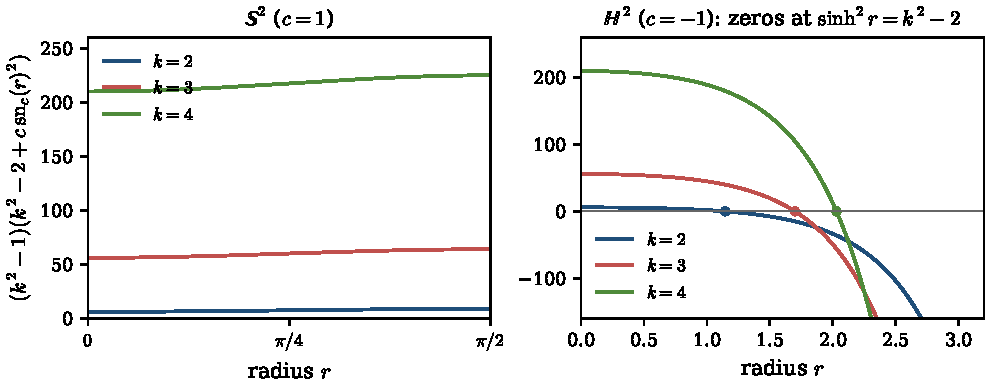
\includegraphics[width=\textwidth]{figures/second_variation.pdf}
\caption{The factor $(k^2-1)(k^2-2+c\,\sn_c(r)^2)$ of the second variation \eqref{eq:Q} for $k=2,3,4$. Left: the unit sphere, where all factors are positive. Right: the hyperbolic plane, where the factor of mode $k$ vanishes at $\sinh^2r=k^2-2$ (dots) and is negative for larger $r$.}
\label{fig:second}
\end{figure}

\begin{theorem}\label{thm:universal}
Let $\gamma_\eps$ be as in Theorem~A and $\mu\in\RR$. Then
\begin{equation}\label{eq:universal}
\E(\gamma_\eps)-\frac{K(\gamma_\eps)^2}{L(\gamma_\eps)}-\mu\,\Delta_c(\gamma_\eps)
=\frac{\pi\eps^2}{S_0^3}\sum_{k\ge2}(k^2-1)\bigl(k^2-1-2\pi\mu S_0^3\bigr)\bigl(a_k^2+b_k^2\bigr)+O(\eps^3).
\end{equation}
Consequently the second-order term is nonnegative for every $u$ if and only if $\mu\le 3/(2\pi S_0^3)=12\pi^2/L_0^3$, where $L_0=2\pi S_0$.
\end{theorem}

\begin{proof}
First we expand $\Delta_c$. Its value and first-order coefficient vanish: $\Delta_c=0$ on circles, and $2L_0L_1-4\pi A_1+2cA_0A_1=2(L_0C_0-K_0S_0)I_0=0$. For the second-order coefficient, Lemma~\ref{lem:expansions} gives
\[
\Delta_2=2L_0L_2+L_1^2-2K_0A_2+cA_1^2=2\pi(J_1-cS_0^2I_2)-2\pi C_0^2I_2+(C_0^2+cS_0^2)I_0^2=2\pi(J_1-I_2)+I_0^2 .
\]
With $u=a_0+v$ this is $2\pi\bigl(\int v'^2-\int v^2\bigr)=2\pi^2\sum_{k\ge2}(k^2-1)(a_k^2+b_k^2)$. By \eqref{eq:cs-split}, the left side of \eqref{eq:universal} equals
\[
\G_c(\gamma_\eps)+\Delta_c\Bigl(\frac{K^2}{L(L^2-\Delta_c)}-\mu\Bigr)
=\G_c(\gamma_\eps)+\eps^2\Delta_2\Bigl(\frac{K_0^2}{L_0^3}-\mu\Bigr)+O(\eps^3),
\]
and $K_0^2/L_0^3=C_0^2/(2\pi S_0^3)$. Adding \eqref{eq:Q}, the coefficient of $a_k^2+b_k^2$ is
\[
\frac{\pi}{S_0^3}(k^2-1)\bigl(k^2-2+cS_0^2+C_0^2-2\pi\mu S_0^3\bigr)=\frac{\pi}{S_0^3}(k^2-1)\bigl(k^2-1-2\pi\mu S_0^3\bigr).
\]
Its minimum over $k\ge2$ is attained at $k=2$, and it is nonnegative if and only if $2\pi\mu S_0^3\le3$.
\end{proof}

\begin{remark}\label{rem:universal}
Two features of \eqref{eq:universal} deserve mention. First, the second variations of the Cauchy--Schwarz gap $\E-K^2/L$ and of the deficit $\Delta_c$ are $\pi S_0^{-3}\sum(k^2-1)^2(a_k^2+b_k^2)$ and $2\pi^2\sum(k^2-1)(a_k^2+b_k^2)$. At circles of equal length, neither depends on $c$. Second, by \eqref{eq:cs-split}, the inequality $\G_c\ge0$ is the choice $\mu=K^2/(L\,A(4\pi-cA))$, whose value at the circle is $K_0^2/L_0^3=(4\pi^2-cL_0^2)/L_0^3$. Theorem~\ref{thm:universal} thus recovers Corollary~\ref{cor:sign}: Gage's coefficient is admissible near the circle if and only if $4\pi^2-cL_0^2\le12\pi^2$. In the plane the admissible range is three times larger than Gage's coefficient, and on the sphere it is larger still.
\end{remark}

\section{The hyperbolic plane}\label{sec:hyperbolic}

In this section $c=-1$, $\sn_{-1}=\sinh$ and $\cs_{-1}=\cosh$. The Gage deficit is
\[
\G_{-1}(\gamma)=\int_\gamma\kappa^2\,ds-\frac{(2\pi+A)^2L}{A(4\pi+A)}.
\]

\begin{theorem}\label{thm:hyp}
Let $r>\arcsinh\sqrt2=\log(\sqrt2+\sqrt3)\approx1.1462$ and let $\gamma_\eps$ be the curve $\rho=r+\eps\cos2\theta$ in $\HH^2$. Then
\[
\G_{-1}(\gamma_\eps)=\frac{3\pi\,(2-\sinh^2r)}{\sinh^3r}\,\eps^2+O(\eps^3).
\]
Hence there is $\eps_0>0$ such that for $0<|\eps|<\eps_0$ the curve $\gamma_\eps$ is a smooth closed curve with $\kappa>1$ and $\G_{-1}(\gamma_\eps)<0$.
\end{theorem}

\begin{proof}
The expansion is \eqref{eq:Q} with $c=-1$, $S_0=\sinh r$, $a_2=1$ and all other coefficients zero, and its leading coefficient is negative. The curvature of $\gamma_\eps$ depends smoothly on $(\eps,\theta)$ and equals $\coth r>1$ at $\eps=0$, so $\kappa>1$ for $|\eps|$ small. By Lemma~\ref{lem:polar} the curve is embedded and bounds a star-shaped domain, which is convex because $\kappa>0$.
\end{proof}

\begin{figure}[htbp]
\centering
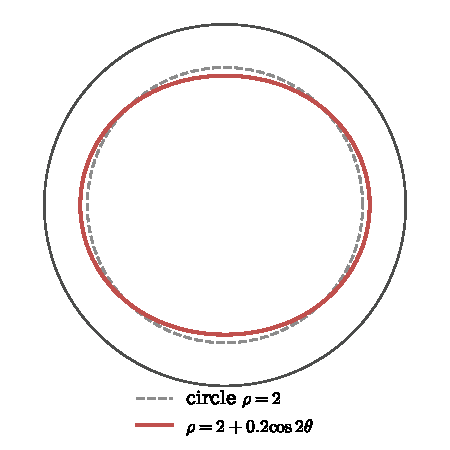
\includegraphics[width=0.42\textwidth]{figures/counterexample.pdf}
\caption{The circle of radius $2$ (dashed) and the curve $\rho=2+0.2\cos2\theta$ (solid) in the Poincar\'e disc. The perturbed curve is convex and violates the hyperbolic Gage inequality: $\int\kappa^2\,ds=24.71919<24.80403=(2\pi+A)^2L/(A(4\pi+A))$.}
\label{fig:counterexample}
\end{figure}

\begin{corollary}\label{cor:hyp-csf}
Let $\gamma_0$ be one of the curves of Theorem~\ref{thm:hyp}, and let $\gamma_t$ be the curve shortening flow starting at $\gamma_0$. Then $I_{-1}(\gamma_t)=L^2/(A(4\pi+A))$ is strictly increasing on $[0,t_0)$ for some $t_0>0$.
\end{corollary}

\begin{proof}
The flow is smooth on some interval $[0,T)$ and $\gamma_t$ is convex for small $t$ \cite{Ga90a,Gr89}. By Proposition~\ref{prop:csf}, $\frac{d}{dt}\log I_{-1}$ equals $-2\G_{-1}(\gamma_0)/L(\gamma_0)>0$ at $t=0$, and it is continuous in $t$.
\end{proof}

Since $A'=-(2\pi+A)\le-2\pi$, the flow becomes singular before time $A(\gamma_0)/2\pi$, and by Grayson's theorem \cite{Gr89} the curves converge to a point. In the computations of Section~\ref{sec:numerics} the ratio, after its initial increase, decreases to $1$ at the extinction time (Figure~\ref{fig:csf}), as it must if the curves become asymptotically circular.

\begin{remark}\label{rem:modes}
By Corollary~\ref{cor:sign}, if $k^2-2<\sinh^2r\le(k+1)^2-2$ then the modes $2,\dots,k$ are unstable, and the circle has $2(k-1)$ independent directions along which $\G_{-1}$ decreases to second order. The first threshold $\sinh^2r=2$ corresponds to $L=2\pi\sqrt2\approx8.886$, $A=2\pi(\sqrt3-1)\approx4.600$ and $K=2\pi\sqrt3$. For general $c<0$ the condition reads $-cL^2>8\pi^2$.
\end{remark}

Table~\ref{tab:hyp} lists some perturbed circles computed as in Section~\ref{sec:numerics}. They include horocyclically convex curves with $\G_{-1}<0$, such as $r=2$, $\eps=0.05$ with $\min\kappa=1.0245$, and curves with larger perturbations, for which the inequality still fails. At $r=1.2$, where mode~$2$ is only slightly unstable ($\sinh^21.2\approx2.28$), the curve with $\eps=0.05$ violates the inequality but the one with $\eps=0.2$ does not. There the higher-order terms dominate. Figure~\ref{fig:csf} shows the computed isoperimetric ratio along two flows; it first increases and then decreases.

\begin{table}[t]
\centering
\small
\caption{Perturbed circles $\rho=r+\eps\cos k\theta$ in $\HH^2$. Here $\Phi=(2\pi+A)^2L/(A(4\pi+A))$, $q_k$ is the coefficient of $\eps^2$ in \eqref{eq:Q}, and $D/\sqrt\Delta$ is the ratio of the two sides of \eqref{eq:L1} minimized over $\lambda$. Values are computed with $8192$ points.}
\label{tab:hyp}
\begin{tabular}{cccrrrrcrrr}
\toprule
$r$ & $k$ & $\eps$ & $L$ & $A$ & $\int\kappa^2ds$ & $\Phi$ & $\int\kappa^2ds/\Phi$ & $\min\kappa$ & $q_k$ & $D/\sqrt\Delta$\\
\midrule
1.0 & 2 & 0.05 & 7.40198 & 3.41834 & 12.75950 & 12.74994 & 1.000750 & 1.1863 & $+3.594$ & 0.991\\
1.0 & 2 & 0.20 & 7.66987 & 3.50947 & 13.33155 & 13.03687 & 1.022604 & 0.4917 & $+3.594$ & 0.819\\
1.0 & 3 & 0.05 & 7.41863 & 3.41834 & 12.99758 & 12.77862 & 1.017135 & 0.9795 & $+87.007$ & 1.568\\
1.2 & 2 & 0.05 & 9.50056 & 5.10061 & 13.66110 & 13.66277 & 0.999878 & 1.1238 & $-0.763$ & 0.850\\
1.2 & 2 & 0.20 & 9.74516 & 5.20755 & 13.93427 & 13.90170 & 1.002343 & 0.7338 & $-0.763$ & 0.738\\
1.2 & 3 & 0.05 & 9.51354 & 5.10061 & 13.76859 & 13.68144 & 1.006370 & 0.9999 & $+34.503$ & 1.365\\
1.5 & 2 & 0.05 & 13.39440 & 8.50668 & 16.33811 & 16.34422 & 0.999626 & 1.0672 & $-2.474$ & 0.658\\
1.5 & 2 & 0.20 & 13.63087 & 8.64562 & 16.48619 & 16.56518 & 0.995232 & 0.8831 & $-2.474$ & 0.598\\
1.5 & 3 & 0.05 & 13.40361 & 8.50668 & 16.37188 & 16.35546 & 1.001004 & 1.0055 & $+6.420$ & 1.067\\
2.0 & 2 & 0.05 & 22.80681 & 17.37016 & 24.53280 & 24.53830 & 0.999776 & 1.0245 & $-2.204$ & 0.413\\
2.0 & 2 & 0.20 & 23.08622 & 17.59236 & 24.71919 & 24.80403 & 0.996579 & 0.9638 & $-2.204$ & 0.388\\
2.0 & 3 & 0.05 & 22.81223 & 17.37016 & 24.53610 & 24.54412 & 0.999673 & 1.0034 & $-3.242$ & 0.673\\
3.0 & 2 & 0.05 & 62.98508 & 57.01334 & 63.60959 & 63.61189 & 0.999964 & 1.0033 & $-0.922$ & 0.154\\
3.0 & 2 & 0.20 & 63.60039 & 57.60795 & 64.18451 & 64.22149 & 0.999424 & 0.9955 & $-0.922$ & 0.148\\
3.0 & 3 & 0.05 & 62.98704 & 57.01334 & 63.60804 & 63.61387 & 0.999908 & 1.0005 & $-2.334$ & 0.252\\
\bottomrule
\end{tabular}
\end{table}

For small curves the evidence points the other way. None of $44{,}755$ random convex curves in $\HH^2$ of length below $2\pi\sqrt2$ violates \eqref{eq:gage-c} (Section~\ref{sec:numerics}).

\begin{question}\label{q:small}
Does every convex curve $\gamma\subset\HH^2$ with $L(\gamma)\le2\pi\sqrt2$ satisfy $\G_{-1}(\gamma)\ge0$?
\end{question}

\section{The sphere}\label{sec:sphere}

In this section $c=1$ and $M_1=\Sph^2\subset\RR^3$ is the unit sphere. The Gage deficit is
\[
\G_1(\gamma)=\int_\gamma\kappa^2\,ds-\frac{(2\pi-A)^2L}{A(4\pi-A)}=\int_\gamma\kappa^2\,ds-\frac{K^2L}{4\pi^2-K^2}.
\]
By Corollary~\ref{cor:sign}(a), every spherical circle of radius $r\in(0,\pi/2)$ is a strict local minimizer of $\G_1$ in the sense made precise there.

\subsection{Polarity}\label{sec:polar}
Let $\gamma$ be a smooth convex curve on $\Sph^2$ parametrized by arclength, $T=\gamma'$ and $n=\gamma\times T$. Then $n$ is the unit normal pointing into $\Omega$, and the frame equations are
\begin{equation}\label{eq:frame}
T'=-\gamma+\kappa n,\qquad n'=-\kappa T .
\end{equation}
The \emph{polar curve} of $\gamma$ is $\gamma^*:=n$. Its trace is the boundary of the polar domain $\Omega^*=\{y\in\Sph^2:\langle y,x\rangle\ge0\text{ for all }x\in\Omega\}$, which is again a compact convex domain in an open hemisphere \cite{Sa42}.

\begin{lemma}\label{lem:polarity}
The polar curve $\gamma^*$ is a smooth convex curve bounding $\Omega^*$. With arclength $s^*$, it satisfies
\[
ds^*=\kappa\,ds,\qquad \kappa^*=\frac1\kappa,\qquad L^*=K=2\pi-A,\qquad A^*=2\pi-L,\qquad (\gamma^*)^*=\gamma .
\]
\end{lemma}

\begin{proof}
By \eqref{eq:frame}, $(\gamma^*)'=-\kappa T$, so $ds^*=\kappa\,ds$ and the unit tangent is $T^*=-T$. The frame $(\gamma,T,n)$ is positively oriented and orthonormal, so the normal of $\gamma^*$ is $n^*=\gamma^*\times T^*=n\times(-T)=T\times n=\gamma$. Moreover
\[
\frac{dT^*}{ds^*}=-\frac{T'}{\kappa}=\frac{\gamma}{\kappa}-n=-\gamma^*+\frac1\kappa\,n^*,
\]
so $\kappa^*=1/\kappa>0$ by \eqref{eq:frame} applied to $\gamma^*$, and $(\gamma^*)^*=n^*=\gamma$. The length is $L^*=\int\kappa\,ds=K=2\pi-A$. The normal $n^*=\gamma$ points into $\Omega^*$, so Gauss--Bonnet for $\Omega^*$ gives $A^*=2\pi-\int\kappa^*\,ds^*=2\pi-\int ds=2\pi-L$.
\end{proof}

\begin{corollary}\label{cor:dual}
For every smooth convex curve $\gamma\subset\Sph^2$,
\[
\G_1(\gamma^*)=\int_\gamma\frac{ds}{\kappa}-\frac{L^2\,(2\pi-A)}{4\pi^2-L^2},\qquad \Delta_1(\gamma^*)=\Delta_1(\gamma).
\]
Consequently \eqref{eq:gage-c} holds for all convex spherical curves if and only if
\begin{equation}\label{eq:dual}
\int_\gamma\frac{ds}{\kappa}\ \ge\ \frac{L^2\,(2\pi-A)}{4\pi^2-L^2}\qquad\text{for all convex curves }\gamma\subset\Sph^2 .
\end{equation}
\end{corollary}

\begin{proof}
We have $\int\kappa^{*2}\,ds^*=\int\kappa^{-2}\kappa\,ds=\int ds/\kappa$ and $2\pi-A^*=L$. By \eqref{eq:4pi2}, $A^*(4\pi-A^*)=4\pi^2-K^{*2}=4\pi^2-L^2$. Moreover $\Delta_1(\gamma^*)=L^{*2}-A^*(4\pi-A^*)=(2\pi-A)^2-4\pi^2+L^2=\Delta_1(\gamma)$. Since $\gamma\mapsto\gamma^*$ is an involution on smooth convex curves, the equivalence follows; $C^2$ curves are handled by approximation.
\end{proof}

Cauchy--Schwarz gives $\int ds/\kappa=\int\kappa^{-2}\,d\sigma\ge L^2/K$ with $d\sigma=\kappa\,ds$, and \eqref{eq:dual} strengthens it by the factor $K^2/(4\pi^2-L^2)\ge1$. In the plane $\int ds/\kappa\ge L^2/2\pi$ is the whole story. On the sphere the two inequalities \eqref{eq:gage-c} and \eqref{eq:dual} are exchanged by polarity. The isoperimetric ratio $I_1(\gamma)=L^2/(4\pi^2-K^2)$ is exchanged with $I_1(\gamma^*)=K^2/(4\pi^2-L^2)$.

\subsection{An \texorpdfstring{$L^1$}{L1} criterion}

\begin{theorem}\label{thm:L1}
Let $\gamma$ be a convex curve in $M_c$ and let $\lambda^*$ be a median of $1/\kappa$ with respect to the measure $d\sigma=\kappa\,ds$. If
\begin{equation}\label{eq:L1-median}
\int_\gamma\bigl|1-\lambda^*\kappa\bigr|\,ds\ \ge\ \sqrt{\Delta_c(\gamma)},
\end{equation}
then $\G_c(\gamma)\ge0$. In particular \eqref{eq:L1} implies $\G_c(\gamma)\ge0$. Moreover $\lambda\mapsto\int|1-\lambda\kappa|\,ds$ attains its minimum at $\lambda^*$.
\end{theorem}

\begin{proof}
Put $x=1/\kappa$, so that $\int x\,d\sigma=L$ and $\sigma(\gamma)=K$. The measure $\sigma$ has no atoms, so we can split the parameter circle into measurable sets $E_1,E_2$ with $\sigma(E_1)=\sigma(E_2)=K/2$, $x\ge\lambda^*$ on $E_1$ and $x\le\lambda^*$ on $E_2$. Let $x_i=(2/K)\int_{E_i}x\,d\sigma$. Then $x_1+x_2=2L/K$ and, since the two sets have equal measure,
\[
x_1-x_2=\frac2K\Bigl(\int_{E_1}(x-\lambda^*)\,d\sigma+\int_{E_2}(\lambda^*-x)\,d\sigma\Bigr)=\frac2K\int|x-\lambda^*|\,d\sigma=\frac2K\int_\gamma|1-\lambda^*\kappa|\,ds .
\]
For an arbitrary $\lambda$ we have $\int|x-\lambda|\,d\sigma\ge\int_{E_1}(x-\lambda)\,d\sigma+\int_{E_2}(\lambda-x)\,d\sigma=\int|x-\lambda^*|\,d\sigma$, again because $\sigma(E_1)=\sigma(E_2)$. Since $\int_\gamma|1-\lambda\kappa|\,ds=\int|x-\lambda|\,d\sigma$, this proves the last assertion. By Jensen's inequality for the convex function $1/x$ on each $E_i$,
\[
\E(\gamma)=\int\frac{d\sigma}{x}\ \ge\ \frac K2\Bigl(\frac1{x_1}+\frac1{x_2}\Bigr)=\frac{K(x_1+x_2)}{2x_1x_2}=\frac{L}{x_1x_2}.
\]
By \eqref{eq:L1-median}, $x_1-x_2\ge2\sqrt{\Delta_c}/K$, hence
\[
x_1x_2=\tfrac14\bigl((x_1+x_2)^2-(x_1-x_2)^2\bigr)\le\frac{L^2-\Delta_c}{K^2}=\frac{A(4\pi-cA)}{K^2},
\]
and therefore $\E\ge K^2L/(A(4\pi-cA))$.
\end{proof}

\begin{proposition}\label{prop:planar-L1}
Every convex plane curve satisfies $\int_\gamma|1-\lambda\kappa|\,ds\ge\sqrt{L^2-4\pi A}$ for all $\lambda\in\RR$. Consequently, by Theorem~\ref{thm:L1}, it satisfies Gage's inequality \eqref{eq:gage}.
\end{proposition}

\begin{proof}
By \cite{Ga90b} there is a point $O$, a positive centre, such that the support function $h$ of $\gamma$ with respect to $O$ satisfies $Lh-A-\pi h^2\ge0$ at every point of $\gamma$. Equivalently, with $u_0=\sqrt{L^2-4\pi A}$,
\[
\Bigl|h-\frac L{2\pi}\Bigr|\le\frac{u_0}{2\pi}.
\]
We may assume $u_0>0$. The function $\phi=(2\pi/u_0)(L/2\pi-h)$ satisfies $|\phi|\le1$, so for every $\lambda$
\[
\int|1-\lambda\kappa|\,ds\ \ge\ \int(1-\lambda\kappa)\,\phi\,ds=\frac{2\pi}{u_0}\Bigl(\frac{L^2}{2\pi}-\int h\,ds-\lambda\Bigl(L-\int\kappa h\,ds\Bigr)\Bigr)=\frac{L^2-4\pi A}{u_0}=u_0 .
\]
Here we used the Minkowski formulas $\int h\,ds=2A$ and $\int\kappa h\,ds=L$, and $\int\kappa\,ds=2\pi$.
\end{proof}

\begin{remark}
In the notation of Green and Osher, the left side of \eqref{eq:L1} at the median is $\int_0^{2\pi}|\rho-\lambda^*|\,d\theta$. Proposition~\ref{prop:planar-L1} is equivalent to the inequality $\rho_1\ge h_+$ between the mean radius of curvature $\rho_1$ over the half of the normal directions where $\rho$ is largest and the larger Steiner root $h_+$ \cite{GO99,PY08,GPY15}. With Theorem~\ref{thm:L1} and Karamata's inequality in place of Jensen's, it yields the Green--Osher inequality for every convex $F$. The proof above, by testing against the support function at a positive centre, is short.
\end{remark}

\begin{proposition}\label{prop:local-L1}
Let $\gamma_\eps$ be as in Theorem~A with $u\notin\spn\{1,\cos\theta,\sin\theta\}$, and set
\[
D(\eps)=\min_{\lambda\in\RR}\int_{\gamma_\eps}|1-\lambda\kappa|\,ds,\qquad
\Lambda(u)=\frac{\min_{t\in\RR}\int_0^{2\pi}|u''+u-t|\,d\theta}{\pi\sqrt{2\sum_{k\ge2}(k^2-1)(a_k^2+b_k^2)}} .
\]
Then $D(\eps)/\sqrt{\Delta_c(\gamma_\eps)}\to\Lambda(u)/\cs_c(r)$ as $\eps\to0$. Moreover $\Lambda(u)\ge1$ for every such $u$, and $\Lambda(\cos2\theta)=2\sqrt6/\pi\approx1.5594$. Consequently:
\begin{enumerate}[label=\textup{(\alph*)}]
\item if $c>0$, then \eqref{eq:L1} holds for $\gamma_\eps$ when $|\eps|$ is small;
\item if $c<0$ and $\cosh(\sqrt{-c}\,r)>2\sqrt6/\pi$, then \eqref{eq:L1} fails for $\gamma_\eps$ with $u=\cos2\theta$ and all small $\eps\ne0$.
\end{enumerate}
\end{proposition}

\begin{proof}
Let $w=u+u''$. From the expansions in the proof of Lemma~\ref{lem:expansions}, uniformly in $\theta$,
\[
\kappa_\eps=\frac{C_0}{S_0}-\eps\,\frac{w}{S_0^2}+O(\eps^2),\qquad ds_\eps=\bigl(S_0+O(\eps)\bigr)\,d\theta .
\]
Write $\lambda=(S_0/C_0)(1+\eps\tau)$. Then $1-\lambda\kappa_\eps=\eps\bigl(w/(S_0C_0)-\tau\bigr)+\eps^2e$ with $|e|\le C(1+|\tau|)$ uniformly for $|\eps|\le1$, hence
\[
\int_{\gamma_\eps}|1-\lambda\kappa_\eps|\,ds_\eps=\frac{|\eps|}{C_0}\int_0^{2\pi}|w-S_0C_0\tau|\,d\theta+O\bigl(\eps^2(1+|\tau|)\bigr).
\]
On the other hand $\int|1-\lambda\kappa|\,ds\ge|L-\lambda K|$, and by Lemma~\ref{lem:expansions} and \eqref{eq:gb}, $L-\lambda K=\eps\bigl(I_0/C_0-2\pi S_0\tau\bigr)+O(\eps^2(1+|\tau|))$. Hence, for $|\eps|$ small enough, $\int|1-\lambda\kappa|\,ds\ge|\eps|\bigl(\pi S_0|\tau|-|I_0|/C_0-1\bigr)$ for every $\tau$. Choose $T$ with $\pi S_0T-|I_0|/C_0-1>(1/C_0)\int|w|\,d\theta+1$. For small $|\eps|$ the values with $|\tau|>T$ then exceed the value at $\tau=0$, so the minimum is attained with $|\tau|\le T$, where the error term is $O(\eps^2)$. Hence $D(\eps)=(|\eps|/C_0)\min_t\int|w-t|\,d\theta+O(\eps^2)$.

The proof of Theorem~\ref{thm:universal} gives $\Delta_c(\gamma_\eps)=2\pi^2\eps^2\sum_{k\ge2}(k^2-1)(a_k^2+b_k^2)+O(\eps^3)$ with a positive coefficient, which proves the limit. The quantity $\Lambda(u)$ does not depend on $c$ or $r$. Taking $c=0$, Proposition~\ref{prop:planar-L1} gives $D(\eps)\ge\sqrt{\Delta_0(\gamma_\eps)}$ for all small $\eps$, hence $\Lambda(u)\ge1$. For $u=\cos2\theta$ we have $w=-3\cos2\theta$, whose median is $0$, so the numerator is $3\int_0^{2\pi}|\cos2\theta|\,d\theta=12$ and $\Lambda=12/(\pi\sqrt6)=2\sqrt6/\pi$. Finally $\cs_c(r)<1$ for $c>0$ gives (a), and (b) follows because the limit $\Lambda(\cos2\theta)/\cosh(\sqrt{-c}\,r)$ is then below $1$.
\end{proof}

For $c=-1$, Proposition~\ref{prop:local-L1} shows that \eqref{eq:L1} fails near circles with $2\sqrt6/\pi<\cosh r<\sqrt3$, where $\G_{-1}$ is still locally nonnegative. Thus \eqref{eq:L1} is strictly stronger than \eqref{eq:gage-c}. Theorem~\ref{thm:L1} also shows that \eqref{eq:L1} fails for every curve of Theorem~\ref{thm:hyp}, since those curves have $\G_{-1}<0$. The last column of Table~\ref{tab:hyp} illustrates both facts.

\begin{remark}\label{rem:fronts}
On $\Sph^2$ the criterion has two geometric forms. For $0<\delta<\pi/2$ let $\gamma^{(\delta)}=\cos\delta\,\gamma+\sin\delta\,n$ be the inner parallel front of $\gamma$ at distance $\delta$, a closed wave front that may have cusps. By \eqref{eq:frame} its derivative with respect to the arclength $s$ of $\gamma$ is $(\cos\delta-\kappa\sin\delta)\,T$, so
\[
\int_\gamma|1-\kappa\tan\delta|\,ds=\frac{\operatorname{length}(\gamma^{(\delta)})}{\cos\delta}.
\]
For $\lambda\le0$ inequality \eqref{eq:L1} is trivial because its left side is at least $L\ge\sqrt{\Delta_1}$. Hence \eqref{eq:L1} says that every inner parallel front of $\gamma$ at distance $\delta$ has length at least $\cos\delta\,\sqrt{L^2-A(4\pi-A)}$. By Lemma~\ref{lem:polarity}, $\int_\gamma|1-\lambda\kappa|\,ds=\int_{\gamma^*}|\kappa^*-\lambda|\,ds^*$ and $\Delta_1(\gamma^*)=\Delta_1(\gamma)$. So \eqref{eq:L1} for all convex spherical curves is equivalent to
\[
\int_\gamma|\kappa-\lambda|\,ds\ \ge\ \sqrt{L^2-A(4\pi-A)}\qquad\text{for all convex }\gamma\subset\Sph^2\text{ and all }\lambda\in\RR,
\]
that is, to a lower bound for the $L^1$ distance from the geodesic curvature to the constants.
\end{remark}

\begin{conjecture}\label{conj:sphere}
Let $\gamma\subset\Sph^2$ be a convex curve.
\begin{enumerate}[label=\textup{(\alph*)}]
\item $\int_\gamma|1-\lambda\kappa|\,ds\ge\sqrt{L^2-A(4\pi-A)}$ for every $\lambda\in\RR$.
\item $\int_\gamma\kappa^2\,ds\ge(2\pi-A)^2L/(A(4\pi-A))$, with equality only for circles. Equivalently, the isoperimetric ratio $L^2/(A(4\pi-A))$ is nonincreasing along the curve shortening flow of every convex spherical curve, and \eqref{eq:dual} holds.
\end{enumerate}
\end{conjecture}

By Theorem~\ref{thm:L1}, part (a) implies the inequality in part (b). The conjecture is supported by Corollary~\ref{cor:sign}, by Proposition~\ref{prop:local-L1} and by the experiments of Section~\ref{sec:numerics}.

\section{Numerical experiments}\label{sec:numerics}

\subsection{Method}
A closed curve is sampled at $N$ equispaced values of a $2\pi$-periodic parameter. Derivatives are computed with the discrete Fourier transform and integrals with the trapezoidal rule; both are spectrally accurate for smooth periodic data. We realize $\Sph^2$ as the unit sphere in $\RR^3$ and $\HH^2$ as the hyperboloid $\{x_1^2+x_2^2-x_3^2=-1,\ x_3>0\}$ in Minkowski space. In both models the geodesic curvature of $x(t)$ is $\det(x,x',x'')/|x'|^3$, with the Euclidean or Minkowski norm of $x'$.

Convex test curves are obtained from planar convex curves $\Gamma$ with support function $H$. For $\Sph^2$ we lift $\Gamma$ to the upper hemisphere by the inverse gnomonic projection, and for $\HH^2$ we lift a curve in the unit disc by the inverse Beltrami--Klein projection. Both projections map straight lines to geodesics, so convex curves lift to convex curves. The random support functions are $H=a(1+sb)$ plus a random translation. Here $b$ is a random trigonometric polynomial of degree at most $8$ with $k$-th coefficient of size about $k^{-p}$, $p\in[1,2.5]$, and $s$ is a uniformly random fraction, up to $0.93$, of the largest amplitude that keeps $\Gamma$ convex. The samples therefore range from nearly circular curves to curves whose radius of curvature almost vanishes somewhere. The enclosed area is computed independently of the curvature, by integrating the area density of the model over the polar angle. The Gauss--Bonnet residual $|K-(2\pi-cA)|$ never exceeded $2.5\cdot10^{-14}$.

We report three ratios, each at least $1$ exactly when the corresponding inequality holds: $\E/\Phi$ with $\Phi$ the right side of \eqref{eq:gage-c}; the relative improvement $\mathcal R=(\E-K^2/L)/(\Phi-K^2/L)$, which by \eqref{eq:cs-split} is at least $1$ exactly when $\G_c\ge0$ and does not degenerate near circles; and $D/\sqrt{\Delta_c}$, where $D=\min_\lambda\int|1-\lambda\kappa|\,ds$ is computed at the $\sigma$-median (Theorem~\ref{thm:L1}).

\subsection{Validation}
For $u=\cos k\theta$ we computed $\G_c(\gamma_\eps)/\eps^2$ at $\eps=10^{-3}$ and $5\cdot10^{-4}$ with $N=1024$, and removed the $O(\eps)$ term by Richardson extrapolation. Table~\ref{tab:validation} compares the results with \eqref{eq:Q}. In all $24$ cases computed (the table shows a selection) the relative error is at most $1.3\cdot10^{-8}$. The expansions of Lemma~\ref{lem:expansions}, the intermediate expansions in its proof, and Theorems~\ref{thm:second} and~\ref{thm:universal} were also verified symbolically with $\sn_c(r)$ and $\cs_c(r)$ treated as symbols subject to \eqref{eq:sncs}, and separately with the explicit functions $\sin$, $\mathrm{id}$ and $\sinh$. As a check of the whole pipeline against known theorems, $10{,}000$ random convex plane curves satisfy Gage's inequality and Proposition~\ref{prop:planar-L1}. Their smallest ratios are $\mathcal R=3.004$ and $D/\sqrt{\Delta_0}=1.423$.

\begin{table}[t]
\centering
\small
\caption{The coefficient of $\eps^2$ in $\G_c(\gamma_\eps)$ for $u=\cos k\theta$: spectral computation versus \eqref{eq:Q}.}
\label{tab:validation}
\begin{tabular}{rrrrrr}
\toprule
$c$ & $r$ & $k$ & numerical & formula \eqref{eq:Q} & relative error\\
\midrule
$1$ & 0.3 & 2 & 762.2565295 & 762.2565295 & $3.7\cdot10^{-11}$\\
$1$ & 0.8 & 3 & 511.6127317 & 511.6127318 & $8.9\cdot10^{-11}$\\
$1$ & 1.3 & 4 & 786.3607908 & 786.3607909 & $4.2\cdot10^{-11}$\\
$0$ & 1.0 & 2 & 18.8495559 & 18.8495559 & $4.3\cdot10^{-11}$\\
$-1$ & 0.5 & 3 & 1195.0994102 & 1195.0994104 & $1.8\cdot10^{-10}$\\
$-1$ & 1.0 & 2 & 3.5938211 & 3.5938211 & $1.1\cdot10^{-9}$\\
$-1$ & 1.5 & 2 & $-2.4737214$ & $-2.4737214$ & $8.8\cdot10^{-10}$\\
$-1$ & 1.5 & 3 & 6.4204387 & 6.4204387 & $1.6\cdot10^{-9}$\\
$-1$ & 2.5 & 3 & $-3.3596527$ & $-3.3596527$ & $4.6\cdot10^{-9}$\\
$-1$ & 2.5 & 4 & $-4.8098883$ & $-4.8098883$ & $1.1\cdot10^{-8}$\\
\bottomrule
\end{tabular}
\end{table}

\subsection{The sphere}
Of $40{,}000$ random support functions, $31{,}565$ produced convex spherical curves, with $N=2048$. All of them satisfy both parts of Conjecture~\ref{conj:sphere}. The smallest values were $\E/\Phi=1+1.8\cdot10^{-9}$, attained near a circle, $\mathcal R=3.007$ and $D/\sqrt{\Delta_1}=1.487$. Table~\ref{tab:sphere} lists extreme shapes computed with $N=16384$ and $N=32768$; the two resolutions agree to a relative accuracy of $3\cdot10^{-6}$ or better. They include very eccentric ellipses, curves close to a great circle, and rounded polygons with nearly flat sides. The observed lower bound $\mathcal R\ge3$ is consistent with Remark~\ref{rem:universal}: near a circle of radius $r$ the ratio $\mathcal R$ tends to $(k^2-1)/\cos^2r\ge3$ in mode $k$.

\begin{table}[t]
\centering
\small
\caption{Extreme convex curves on $\Sph^2$ (lifts of planar curves by the inverse gnomonic projection). $\Phi=(2\pi-A)^2L/(A(4\pi-A))$, $\mathcal R=(\E-K^2/L)/(\Phi-K^2/L)$, $D=\min_\lambda\int|1-\lambda\kappa|\,ds$.}
\label{tab:sphere}
\begin{tabular}{lrrrrrr}
\toprule
curve & $L$ & $A$ & $\int\kappa^2ds$ & $\Phi$ & $\mathcal R$ & $D/\sqrt{\Delta_1}$\\
\midrule
ellipse $2:1$ & 5.18000 & 2.51640 & 4.3207 & 2.9062 & 9.47 & 2.342\\
ellipse $8:1$ & 5.98534 & 3.05974 & 14.1379 & 2.1381 & 30.85 & 2.119\\
ellipse $20:1$ & 6.16348 & 3.12392 & 35.0209 & 2.0855 & 71.65 & 2.050\\
ellipse $10:1$, small & 5.64187 & 1.76001 & 46.3051 & 6.0690 & 17.47 & 1.497\\
off-centre ellipse & 3.15713 & 0.78085 & 12.9199 & 10.3866 & 4.18 & 1.691\\
small ellipse, far from the pole & 0.08998 & 0.00047 & 1005.2030 & 595.1862 & 3.62 & 1.394\\
rounded triangle, small & 0.53011 & 0.01457 & 2877.3025 & 113.8840 & 70.51 & 1.653\\
rounded triangle, medium & 4.01252 & 1.06035 & 301.4154 & 8.9712 & 135.58 & 1.995\\
rounded triangle, large & 6.09686 & 4.42894 & 32.4010 & 0.5816 & 1798.14 & 5.659\\
rounded square, medium & 4.24021 & 1.43733 & 240.8348 & 6.2246 & 342.69 & 2.954\\
rounded pentagon, large & 6.14853 & 4.91273 & 13.4791 & 0.3071 & 7943.81 & 13.364\\
\bottomrule
\end{tabular}
\end{table}

\subsection{The hyperbolic plane}
Of $60{,}000$ random support functions in the Klein disc, $47{,}270$ produced convex curves with $N=1024$. The $44{,}755$ curves with $L<2\pi\sqrt2$ all satisfy \eqref{eq:gage-c}, with smallest ratio $\E/\Phi=1+3.7\cdot10^{-9}$. Of the $2{,}515$ curves with $L\ge2\pi\sqrt2$, $282$ violate it, and the smallest ratio was $0.9617$. Table~\ref{tab:hyp} was computed with $N=8192$.

\subsection{The curve shortening flow}
For polar graphs, the flow with normal speed $\kappa$ is equivalent to $R_t=-\kappa\sqrt{R'^2+S^2}/S$. We integrate this equation with $N=128$ Fourier modes, $2/3$ dealiasing and the classical Runge--Kutta method, with the time step $0.35\cdot2.78\,\min S^2/(N/2)^2$, below the explicit stability limit. Figure~\ref{fig:csf} shows the results.
\begin{itemize}
\item In $\HH^2$, starting from $\rho=2+0.2\cos2\theta$, the ratio $I_{-1}$ rises from $1.00454$ to $1.01092$ at $t\approx0.79$, where $\G_{-1}$ changes sign. It then decreases to $1+1.8\cdot10^{-5}$ when the area has dropped to $0.05$, at $t=1.327$.
\item Starting from the horocyclically convex curve $\rho=1.6+0.05\cos2\theta$ ($\min\kappa=1.055$), $I_{-1}$ rises from $1.000664$ to $1.000905$ at $t\approx0.40$.
\item On $\Sph^2$, starting from the lift of the ellipse $x^2+4y^2=1$, the ratio $I_1$ decreases monotonically from $1.1220$ to $1+4\cdot10^{-6}$, and $\G_1\ge8.8\cdot10^{-4}$ along the flow.
\end{itemize}

\begin{figure}[t]
\centering
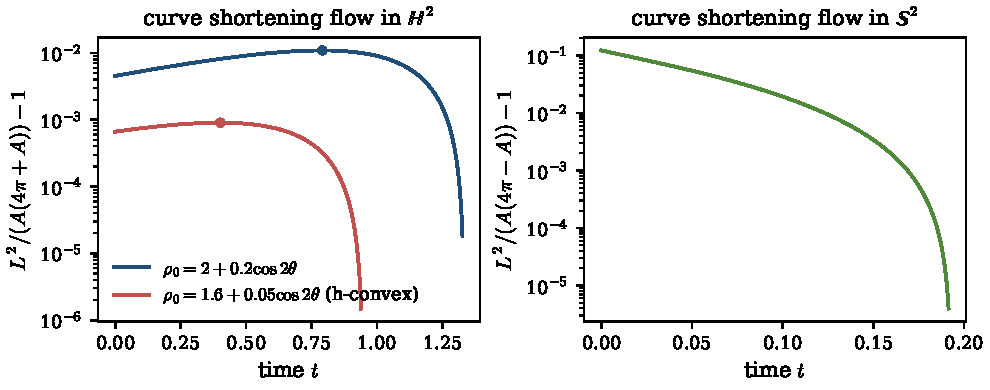
\includegraphics[width=\textwidth]{figures/csf.pdf}
\caption{The isoperimetric ratio minus one along the curve shortening flow. Left: two convex curves in $\HH^2$; the ratio increases until the Gage deficit changes sign (dots), then decreases to $1$. Right: a convex curve on $\Sph^2$, where the ratio decreases monotonically.}
\label{fig:csf}
\end{figure}

\section{Further questions}\label{sec:questions}

\begin{enumerate}[label=\textup{(\arabic*)}]
\item Prove Conjecture~\ref{conj:sphere}. On the sphere, the obstacle to adapting the planar proof of Proposition~\ref{prop:planar-L1} is that no support-type function has both $\int(\cdot)\,ds$ and $\int\kappa(\cdot)\,ds$ determined by $L$ and $A$. For the spherical support function $p=\langle o,n\rangle$ with respect to a point $o\in\Omega$, the planar Minkowski formulas $\int h\,ds=2A$ and $\int\kappa h\,ds=L$ become
\[
\int_\gamma p\,ds=2\int_\Omega\langle x,o\rangle\,dA,\qquad \int_\gamma\kappa p\,ds=\int_\gamma\langle x,o\rangle\,ds,
\]
and neither right side is determined by $L$ and $A$.
\item Answer Question~\ref{q:small}, and determine the largest function $\mu_c(L,A)$ for which $\int\kappa^2\,ds\ge K^2/L+\mu_c(L,A)\,\Delta_c$ holds for all convex curves in $M_c$. Theorem~\ref{thm:universal} shows that $\mu_c\le12\pi^2/L^3$ near circles.
\item In all our planar and spherical samples $\mathcal R\ge3$, and $3$ is the local optimum (Remark~\ref{rem:universal}). In the plane, the inequality $\mathcal R\ge3$ reads
\[
\int_\gamma\kappa^2\,ds\ \ge\ \frac{3\pi L}{A}-\frac{8\pi^2}{L},
\]
which strengthens Gage's inequality by $2\pi(L^2-4\pi A)/(LA)$. For planar ellipses with axis ratio $q$ we found $\mathcal R\to3$ as $q\to1$, $\mathcal R=3.33$ at $q=2$ and $\mathcal R=68.3$ at $q=100$. Does this inequality hold for every convex plane curve, and $\mathcal R\ge3$ for every convex spherical curve?
\item The proof that convex plane curves become circular \cite{Ga84,GH86} starts from the monotonicity of the isoperimetric ratio. In $\HH^2$ the ratio $I_{-1}$ can increase for large curves. Is there a monotone quantity for convex curves in $\HH^2$, sharp on circles, that can replace it?
\end{enumerate}

\begin{thebibliography}{ZMZC12}

\bibitem[AB11]{AB11}
B.~Andrews and P.~Bryan, \emph{Curvature bound for curve shortening flow via distance comparison and a direct proof of Grayson's theorem}, J. Reine Angew. Math. \textbf{653} (2011), 179--187.

\bibitem[Be05]{Be05}
F.~Bernstein, \emph{\"Uber die isoperimetrische Eigenschaft des Kreises auf der Kugeloberfl\"ache und in der Ebene}, Math. Ann. \textbf{60} (1905), 117--136.

\bibitem[CZ01]{CZ01}
K.-S. Chou and X.-P. Zhu, \emph{The Curve Shortening Problem}, Chapman \& Hall/CRC, Boca Raton, FL, 2001.

\bibitem[dC76]{dC76}
M.~P. do~Carmo, \emph{Differential Geometry of Curves and Surfaces}, Prentice-Hall, Englewood Cliffs, NJ, 1976.

\bibitem[Ga83]{Ga83}
M.~E. Gage, \emph{An isoperimetric inequality with applications to curve shortening}, Duke Math. J. \textbf{50} (1983), 1225--1229.

\bibitem[Ga84]{Ga84}
M.~E. Gage, \emph{Curve shortening makes convex curves circular}, Invent. Math. \textbf{76} (1984), 357--364.

\bibitem[Ga90a]{Ga90a}
M.~E. Gage, \emph{Curve shortening on surfaces}, Ann. Sci. \'Ecole Norm. Sup. (4) \textbf{23} (1990), 229--256.

\bibitem[Ga90b]{Ga90b}
M.~E. Gage, \emph{Positive centers and the Bonnesen inequality}, Proc. Amer. Math. Soc. \textbf{110} (1990), 1041--1048.

\bibitem[Ga24]{Ga24}
M.~E. Gage, \emph{A new trick for Santal\'o's integral geometric proof of the strong Bonnesen inequality}, arXiv:2406.01308, 2024.

\bibitem[GH86]{GH86}
M.~Gage and R.~S. Hamilton, \emph{The heat equation shrinking convex plane curves}, J. Differential Geom. \textbf{23} (1986), 69--96.

\bibitem[GPY15]{GPY15}
L.~Gao, S.~Pan and Y.~Yang, \emph{Some notes on Green--Osher's inequality}, J. Math. Inequal. \textbf{9} (2015), 369--380.

\bibitem[GO99]{GO99}
M.~Green and S.~Osher, \emph{Steiner polynomials, Wulff flows, and some new isoperimetric inequalities for convex plane curves}, Asian J. Math. \textbf{3} (1999), 659--676.

\bibitem[Gr87]{Gr87}
M.~A. Grayson, \emph{The heat equation shrinks embedded plane curves to round points}, J. Differential Geom. \textbf{26} (1987), 285--314.

\bibitem[Gr89]{Gr89}
M.~A. Grayson, \emph{Shortening embedded curves}, Ann. of Math. (2) \textbf{129} (1989), 71--111.

\bibitem[Kl07]{Kl07}
D.~A. Klain, \emph{Bonnesen-type inequalities for surfaces of constant curvature}, Adv. in Appl. Math. \textbf{39} (2007), 143--154.

\bibitem[Os78]{Os78}
R.~Osserman, \emph{The isoperimetric inequality}, Bull. Amer. Math. Soc. \textbf{84} (1978), 1182--1238.

\bibitem[PY08]{PY08}
S.~Pan and J.~Yang, \emph{On a non-local perimeter-preserving curve evolution problem for convex plane curves}, Manuscripta Math. \textbf{127} (2008), 469--484.

\bibitem[Sa42]{Sa42}
L.~A. Santal\'o, \emph{Integral formulas in Crofton's style on the sphere and some inequalities referring to spherical curves}, Duke Math. J. \textbf{9} (1942), 707--722.

\bibitem[Sc39]{Sc39}
E.~Schmidt, \emph{\"Uber das isoperimetrische Problem im Raum von $n$ Dimensionen}, Math. Z. \textbf{44} (1939), 689--788.

\bibitem[XZZ15]{XZZ15}
W.~Xu, J.~Zhou and B.~Zhu, \emph{On Bonnesen-type inequalities for a surface of constant curvature}, Proc. Amer. Math. Soc. \textbf{143} (2015), 4925--4935.

\bibitem[ZMZC12]{ZMZC12}
C.~Zeng, L.~Ma, J.~Zhou and F.~Chen, \emph{The Bonnesen isoperimetric inequality in a surface of constant curvature}, Sci. China Math. \textbf{55} (2012), 1913--1919.

\end{thebibliography}

\end{document}
